%%%%%%%%%%%%%%%%%%%%%%%%%%%%%%%%%%%%%%%%%%%%%%%%%%%%%%%%%%%%%%%%%%%%%%%%
%                                                                      %
%     File: Thesis_Background.tex                                      %
%     Tex Master: Thesis.tex                                           %
%                                                                      %
%     Author: Andre C. Marta                                           %
%     Last modified:  4 Mar 2024                                       %
%                                                                      %
%%%%%%%%%%%%%%%%%%%%%%%%%%%%%%%%%%%%%%%%%%%%%%%%%%%%%%%%%%%%%%%%%%%%%%%%

\chapter{Literature Review}
\label{chapter:literaturereview}


%%%%%%%%%%%%%%%%%%%%%%%%%%%%%%%%%%%%%%%%%%%%%%%%%%%%%%%%%%%%%%%%%%%%%%%%
\section{Space Race and Vehicles Reusability}
\label{section:spacerace_reusability}

\textcolor{blue}{Procura pelo espaço}

\textcolor{blue}{Baixo custo de missões, reutilização de estágios}

\textcolor{blue}{Problema de reentrada}

\textcolor{blue}{Novas tecnologias - falar aqui das tecnologias atuais}

%%%%%%%%%%%%%%%%%%%%%%%%%%%%%%%%%%%%%%%%%%%%%%%%%%%%%%%%%%%%%%%%%%%%%%%%
\section{Autorotation for Space Vehicles}
\label{section:autorotation_vehicles}

Using an unpowered rotary wind as an aerodynamic decelerator for spacecraft recovery from a space mission is not a new concept. More than 80 years ago, the first studies were performed, but rapidly the concepts lost interest \textcolor{purple}{encontrar esta referência}. Years after it gained new enthusiasts and some recent projects were published. This section assesses the evolution of the use of Autorotation for Spacecraft.

\subsection{Rotary Wing Recovery System In the Early Ages of Space Exploration}

Over the years some studies have been published focusing on using rotary wings as a concept for vehicle recovery. Ricardo A. Diaz-Silva in \cite{diaz-silva_rotary_2013}, states that early concepts date 1947, when Igor Bensen, from the General Electric Co, published a report titled \textit{Development of Rotochute Rotary Wing Air Brake}. In its work, Bensen developed a device known as Rotochute (fig \ref{fig:rotochute_prototype}) which is a result of merging two keywords: rotor and parachute. The main objective of this device was to develop an aerodynamic decelerator for high-altitude rockets. This device was at the time studied at a supersonic wind tunnel to understand reentry effects. 

\begin{figure}[!htb]
    \centering
    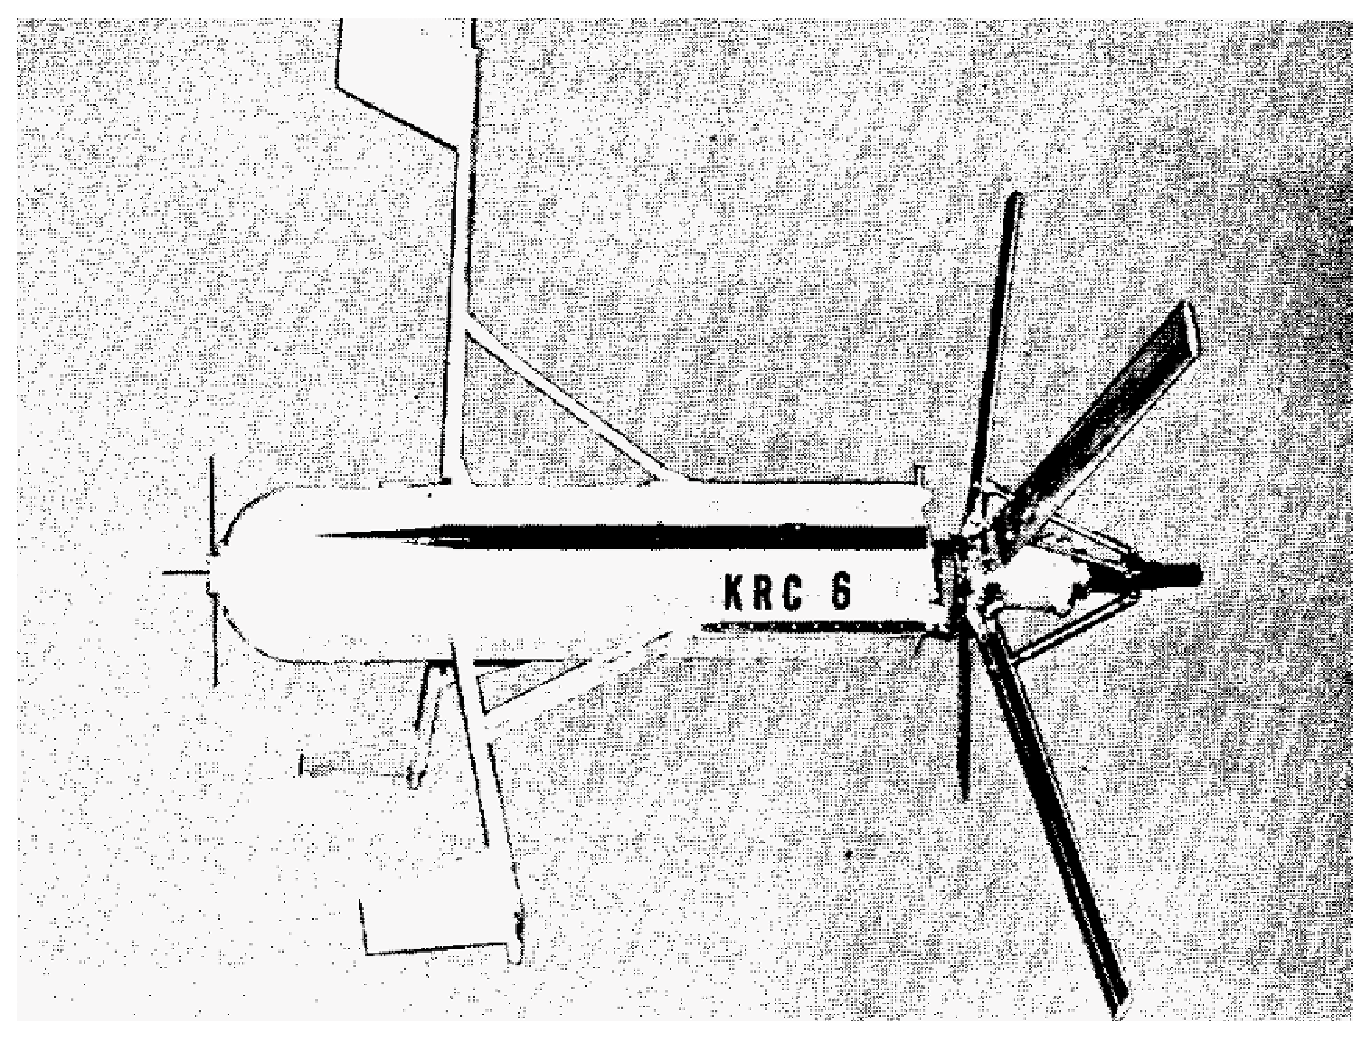
\includegraphics[width=8cm]{Figures/literature_review/rotochute_prototype.eps}
    \caption{KRC-6 Rotochute Flight Test Vehicle}
    \label{fig:rotochute_prototype}
\end{figure}

Also, Kaman Corporation got involved in the rotochute design in the 50s decade and the \gls{nasa} spent some attention studying the proposed system in the 60's, never putting it into practice once all Apollo Missions \cite{noauthor_apollo_nodate} were accomplished by recovering the crew capsule with parachutes landing on the ocean. Important authors in this decade working on the topic, cited in \cite{diaz-silva_rotary_2013}, were Rodney Wernicke from the Bell Helicopter Company, 1957, Justin J. Barzda from Kaman Corporation, 1964, and M. Kretz from the Giravions Dorand Co. in France, 1966. These authors made a substantial original contribution to the area, it is important to comprehend the main ideas of this system by providing a brief overview of their work.

Wernicke published \textit{Preliminary Tests of Model Spacecraft Rotor Landing System} where a three-bladed model was used as able to reduce the vehicle descent axial velocity from supersonic regime to subsonic glide. In its work, Wernicke studied the influence of collective pitch on the model's performance.

On the other hand, Barzda published \textit{Rotor for Recovery} were fixed and telescoping span blades, rotor diameters ranging from 0.3 to 7.3 meters, payloads 2.7 to 408 kg, and rates of descent as low as 6 m/s were points of experimental tests. Barzda did the experimental investigation of deployment from jet aircraft and from a cannon-fired flare shell at  Mach numbers 0.98 and 1.2, respectively. From this investigation, drag and lift coefficients, glide ratios, and cyclic and collective flare performance were crucial results, necessary for the advancement of the concept.

\textit{Space Rotor: A European Project for Recovery of Heavy Launch Vehicles} was published by Kretz and registered a patent. His design aimed to help spacecraft return from orbit by using rotors that could be deployed before re-entry. The system offered benefits like better flight stability, longer range, and precise, soft landings, making reusable launch vehicles possible.

From a historical perspective, Diaz-Silva \cite{diaz-silva_rotary_2013} also makes reference to a Sovietic interest in this system for its Soyuz capsule recovery system, but no references can be found.

\subsection{Recent Projects}
\label{sec:recent_projects}


In recent years, new developments have been published about using rotary wings for recovery space vehicles. The publications show completely different results from the early concepts once the computation technologies have also evolved over the years. It allows researchers to gain deep knowledge of the autorotation phenomena throw computational simulations. Also, conceptual model vehicles were possible to be built with onboard computers to get data from experimental flights due to electronics development.

\subsubsection{\gls{armada}}

A fundamental state-of-the-art project was started to be developed in 2008  by the \gls{esa}, GMV, the University of Bologna and the European Aeronautic \gls{EADS}. The so-called \gls{armada} project \cite{noauthor_armada_nodate} is an \gls{edls}. Its relevance in the field is significant once many other projects were published and taken as reference \gls{armada} project. 

 In the proposed system of \gls{armada} (figure \ref{fig:armada_concept}) a rotor is connected to a conventional helicopter control system, which in turn is mounted on the structure that supports the payload. The deployment process occurs in several stages. Initially, body flaps extend to stabilize the vehicle during deployment. Following this, the rotor blades are deployed using a cable to minimize stress on the joints. 

\begin{figure}[!htb]
    \centering
    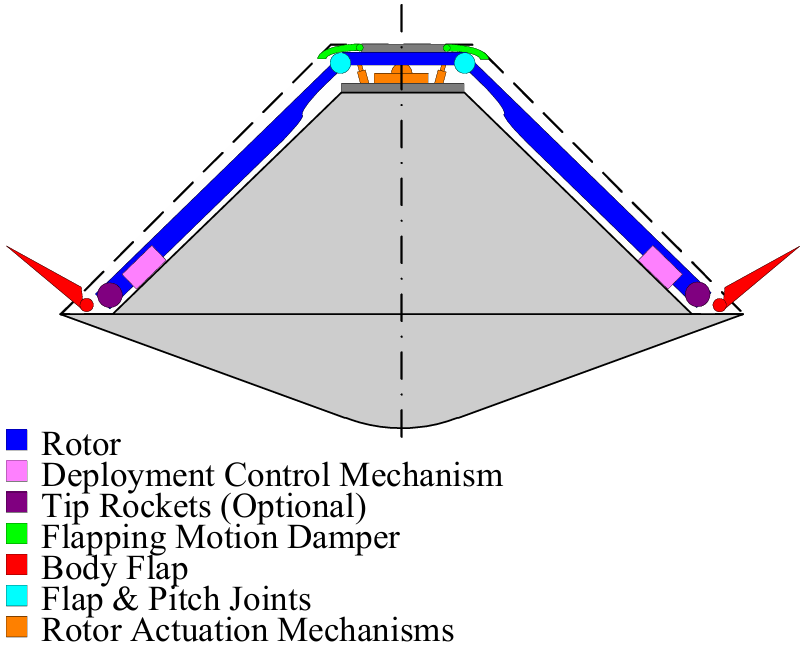
\includegraphics[width=8cm]{Figures/literature_review/armada_concept_vehicle.png}
    \caption{ARMADA Autorotation system concept, from \cite{noauthor_armada_nodate} }
    \label{fig:armada_concept}
\end{figure}

During the deployment, the blades are set to a zero-lift configuration to prevent rotation, with an additional braking system on the rotor shaft ensuring no movement. Once the blades are fully deployed, the retention cables are released, the rotor brake is disengaged, and the collective pitch of the blades is adjusted to allow the rotor to spin. As the lander crosses a predetermined Mach number, centrifugal force extends the telescopic blades, which were initially held in a retracted position by a cable. From this point, the lander descends in its fully deployed state, reaching an equilibrium descent velocity. Just before landing, a flare manoeuvre is executed to further reduce both vertical and horizontal velocities for a safe touchdown.

In \cite{noauthor_armada_nodate}, the deployment phase is further addressed by considering different types of rotor deployment systems. Using a single-piece blade rotor is small and suitable for thicker atmospheres, while a telescopic blade rotor features extendable sections for easy deployment using internal cables. Inflatable blade rotors are lightweight and compact but store less kinetic energy, limiting their manoeuvrability. Foldable blade rotors require precise locking mechanisms to ensure structural stiffness and flexible blade rotors are stabilized through reefing lines, stiffeners, or centrifugal forces in their deployed state. To achieve the best deployment, the authors state that "Any deployment system that can modify the blade length in-flight is highly desirable since this allows an easy method of reefing.", proposing more suitable telescopic blades.

\gls{armada} concepts performance is done using simulations and wind tunnel experiments. Starting with the software tools, figure \ref{fig:armada_software}, uses a divide and conquer approach in which a Performance Database (PD) and an Integrated Parametric Design  Tool (IPDT). To resume how it works, de PD is in simple words a tabe with rotor parameters under specific conditions and de IPDT is interface sheets that interact with the database.

\begin{figure}[!htb]
    \centering
    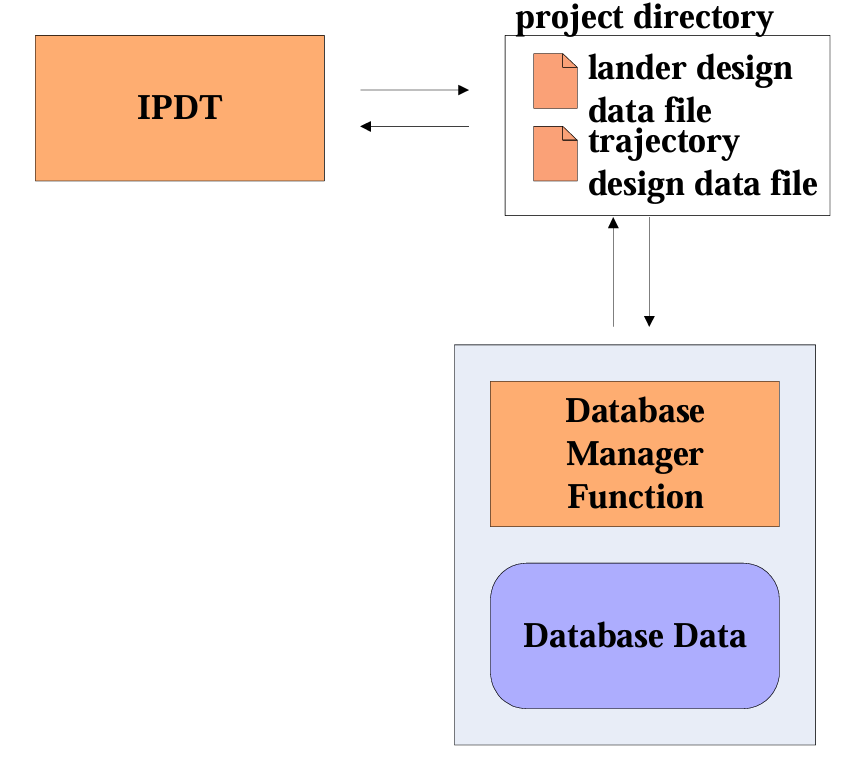
\includegraphics[width=6cm]{Figures/literature_review/armada_software.png}
    \caption{ARMADA concept software, from \cite{noauthor_armada_nodate} }
    \label{fig:armada_software}
\end{figure}

For the experimental tests, a small-scale model, presented in figure \ref{fig:armada_windtunnel} is used. For the supersonic deployment model, figure \ref{fig:armada_supersonic_model}, the S-1 supersonic/transonic wind tunnel 
at Von Karman Institute of Fluid Dynamics was used to test it to Mach number up to 2. For the subsonic regime, the model is tested in the wind tunnel of the Applied Aerodynamic Laboratory of the University of Bologna.

\begin{figure}[!htb]
    \centering
    \subfloat[Supersonic deployment model\label{fig:armada_supersonic_model}]{
        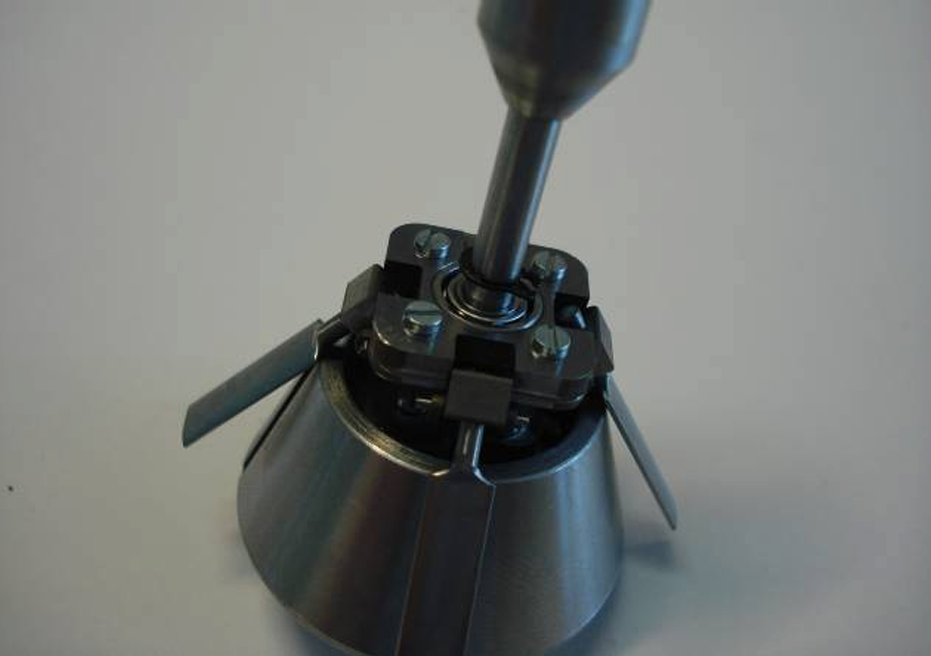
\includegraphics[height=6cm]{Figures/literature_review/armada_supersonic_model.png}
    }\hfill
    \subfloat[Subsonic reefing model\label{fig:aircraft2}]{
        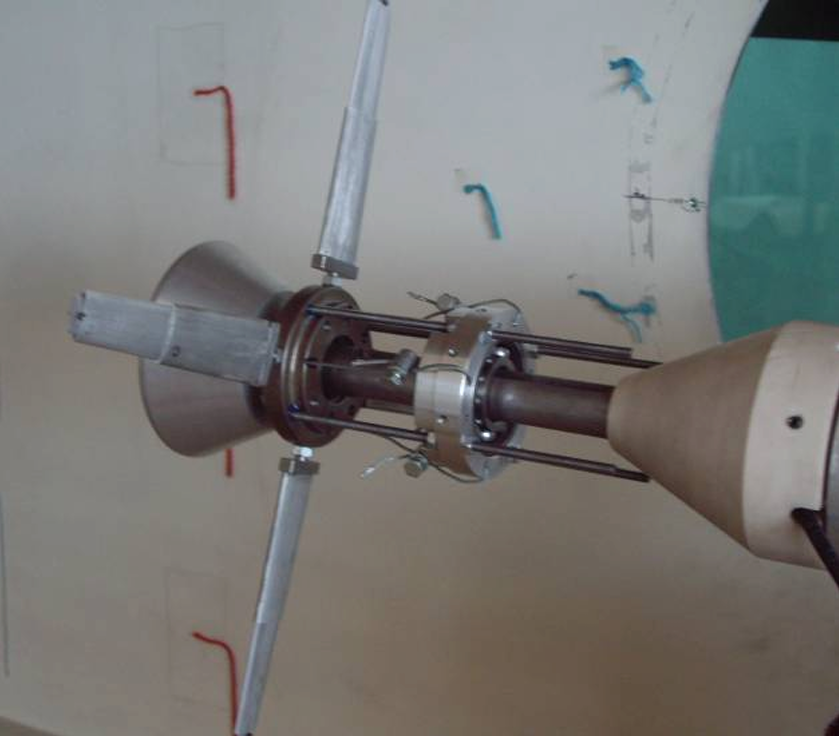
\includegraphics[height=6cm]{Figures/literature_review/armada_subsonic_model.png}
    }
    \caption{ARMADA concepts under different fight conditions}
    \label{fig:armada_windtunnel}
\end{figure}

As results of the study \cite{noauthor_armada_nodate}, show an equilibrium descent velocity that can be obtained with the type of design presented is about 30-40 $m/s$ and was found that this terminal velocity cannot be reduced by increasing the rotor size, and the mass of the rotor itself becomes an important contributor to the overall mass of the vehicle. About this point an essential remark is made:  the mass of the recovery system remains attached to the vehicle, but in traditional systems some mass gets ejected (parachutes) or burnt (propellant). In terms of aerodynamic performance, the distinction between stalled and unstalled operation is evident in the rotor drag coefficient and descent velocity. In installed conditions, the rotor drag coefficient ranges from 1 to 1.25, with a descent velocity of approximately 31 $m/s$. Conversely, when stalled, the rotor drag coefficient drops to around 0.25, and the descent velocity increases significantly to about 80 $m/s$. Furthermore, \gls{armada} faces mechanical challenges, including rotor mass, complexity, descent velocity, and vibration issues. Future solutions may involve improved materials and structures, integrated control systems, and the consideration of additional braking mechanisms.

ARMADA's performance does not justify short-term adoption compared to traditional \gls{edls}. Further research on these approaches is necessary. Overall, ARMADA presents a promising alternative for EDL systems on Earth, Venus, or Titan in the medium to long term.



\subsubsection{Hummingbird}

Further investigation takes to another conceptual project. An undergraduate research project called Project Hummingbird \cite{maurer_project_nodate} aims to launch and recover a sounding rocket with a safe landing achieved by a rotor recovery mechanism. The effort aims to introduce a novel approach to booster recovery that minimizes fuel requirements, streamlines the system, and lowers launch costs.

With foldable rotor blades and an internally stored rotor hub, the system is designed to launch to a height of 2,700 meters. A little parachute will pop out of the nose cone's tip at apogee, allowing the rocket to be oriented with its nose facing upwards. The nose cone will separate in its entirety upon correct alignment. The rotor blades will then immediately deploy and start to revolve on their own, slowing the rocket's descent speed. The rotor will execute a flare movement as the rocket gets closer to the ground to guarantee a safe landing. There will be a flight computer monitoring the rocket's direction and fall. If the rotor blades fail to sufficiently slow down the drop, an emergency parachute will deploy.

\begin{figure}[!htb]
    \centering
    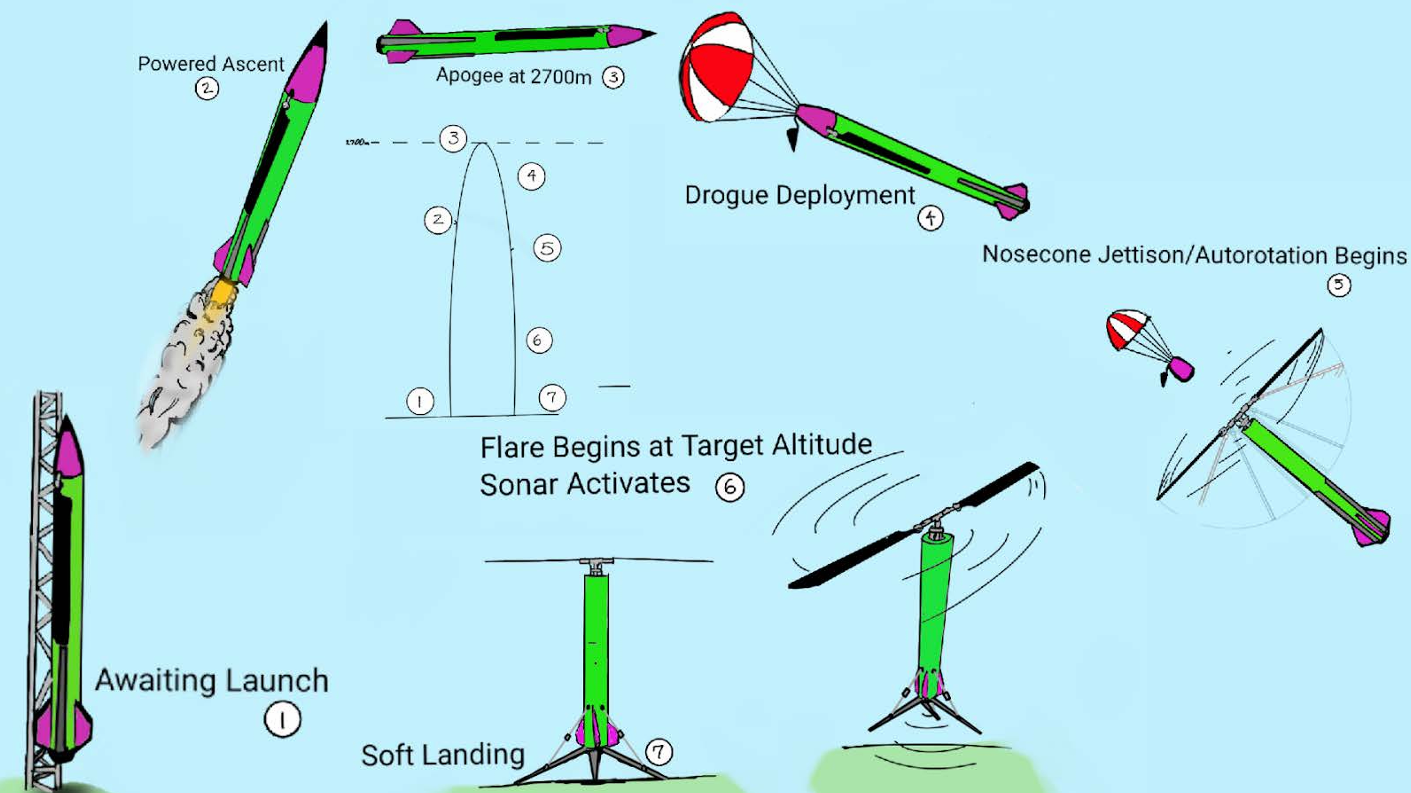
\includegraphics[width=10cm]{Figures/literature_review/Hummingbird_operation.png}
    \caption{Concept of Operation of Project Hummingbird, from \cite{maurer_project_nodate}}
    \label{fig:Hummingbird_operation}
\end{figure}

This project demonstrates an alternative application of rotary wings as a recovery system and introduces a useful hybrid system that combines parachutes and rotary wings. This combination could be crucial if the vehicle is not in the correct position during rotor deployment. Additionally, higher velocities during the deployment phase may result in increased structural stresses, as noted in \cite{noauthor_armada_nodate}.

\subsubsection{DEADALUS}

Riegler et al. developed a prototype \cite{riegler_daedalus_2018} aiming for Earth atmospheric research but also for other \gls{leo} missions. In this work, the authors state that new and safe technologies are needed in the field, proposing a self-stabilizing, free-falling unit, capable of measuring and distributing atmospheric data during descension \cite{riegler_daedalus_2018}. For accomplished the teams goal's, they started by develop the rocket prototype called REXUS, presented in figure 3. 


\begin{figure}[!htb]
    \centering
    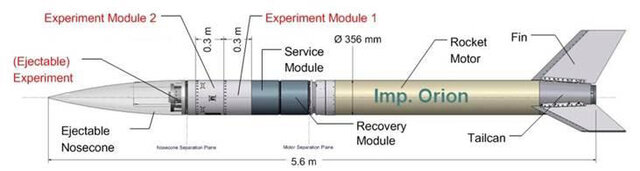
\includegraphics[width=10cm]{Figures/literature_review/REXUS-Rocket-composition_W640.jpg}
    \caption{REXUS Rocket composition, from \cite{riegler_daedalus_2018}}
    \label{fig:rexus_rocket}
\end{figure}

On the REXUS prototype a set o  \gls{ffu} so called SpaceSeeds, are placed inside the REXUS cone, figure \ref{fig:ffu_rexus_inside} and will be injected once the rocket reaches its apogee. This SpaceSeeds are the intereste key point of DEADALUS project on the scope of the use of rotary wings under autorotation phenomena as a recovery system for spacecraft. Figure \ref{fig:ffu_rexus_model} presents a SpaceSeed prototype is presented with four-bladed rotor and a conical main body.



\begin{figure}[!htb]
    \centering
    \subfloat[SpaceSeeds placement inside REXUS's cone, from \cite{noauthor_daedalus_nodate}\label{fig:ffu_rexus_inside}]{
        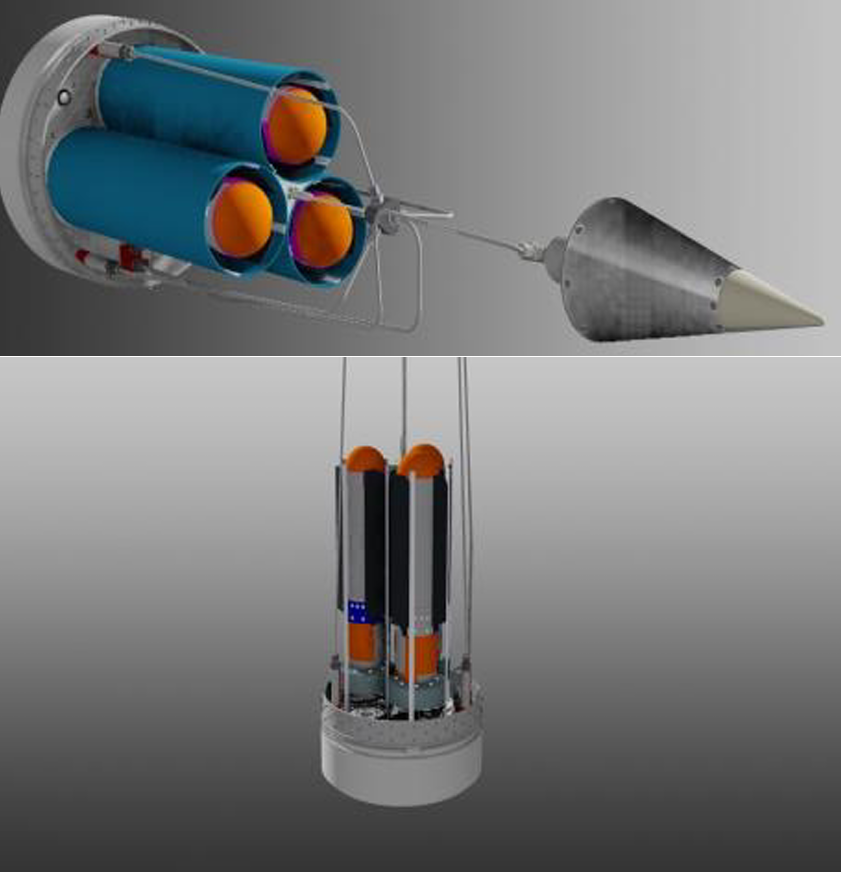
\includegraphics[height=7cm]{Figures/literature_review/ffu_rexus.png}
    }\hfill
    \subfloat[SpaceSeed protoype, from \cite{riegler_project_nodate}\label{fig:ffu_rexus_model}]{
        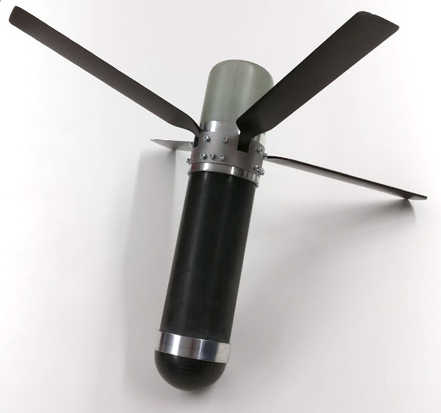
\includegraphics[height=7cm]{Figures/literature_review/space_seed_prototype.png}
    }
    \caption{\gls{ffu} SpaceSeeds used in DEADALUS project}
    \label{fig:daedalus_ffu}
\end{figure}

The development and construction of the space are further presented by Riegler et al. in \cite{riegler_project_nodate}. In this study, the authors explain in better detail the aerodynamic characteristics and software and telemetry information and electronics and its \gls{orbc}. Using the paper words, the \gls{orbc} is the interface between the \gls{rxsm} and the SpaceSeeds, so it is important to refer to it. 

Another important aspect of the project is the mechanical setup. Although it is not the main subject of this study, it is important to highlight the necessity of other components in \cite{riegler_project_nodate} technology. Related to this work two key points are presented: the deployment mechanism which is a crucial aspect of the project once it is necessary to separate the SpaceSeeds from the launcher; the second important point is the wings folding mechanism. The latest mechanical components are not a key point for this study, but it is important to take into consideration, that for spacecraft recovery the blades must be kept inside the vehicle during the launch phase. The blades should only open, unfold or any other way of deploy during the descent phase.

For the mechanical setup, the authors found some mechanical challenges that one must take into consideration: flight loads, especially in the transonic regime, minimum weight, volumetric constraints, natural aerodynamic stability, antenna positioning, radio translucent materials at corresponding areas and landing shock loads.

Finally and more important, is the flight tests. In \cite{riegler_project_nodate} the authors presented a set of different simulation and real flight tests showing good accuracy from computational model and real-flight data. A deeper look at this data is taken in section \textcolor{blue}{meter aqui referência à secção de validação} in which the data is used to validate the computational model presented in this.

From the same authors \cite{mehringer_suborbital_2022} and \cite{bergmann_daedalus_2024} are two more recent publications about the DEADALUS project, in this case, the second version. In thiese papers, some improvements are made to the setup but no available data is presented for comparison.


\subsection{Why using rotary wings for space vehicle recovery?}

\textcolor{blue}{comparação}

To understand why using a rotary wing is a key advantage in space exploration, one can get back to Barzda's work \cite{barzda_rotors_1964} where it is answered. This analysis is mainly done by connecting an already known application of autorotation: helicopters autorotation mandatory manoeuvre in case of power losses \cite{federal_aviation_administration_helicopter_2021}. As helicopters, this is a weatherproof system that can perform under icing or stormy conditions. Another important advantage is the fast and precise deployment over a wide range of speeds. Retardation force builds up rapidly when body orientation is adequate. This allows for recovery, for example, the launcher, when it is necessary to abort the mission in the middle flight to save human lives or payload. A rotary wing is a controllable system, meaning that the pilot can use flight controls to control the vehicle trajectory and rate of descent \cite{federal_aviation_administration_helicopter_2021}. This is an important feature of this system once it is possible to make a safe landing at the intended landing site.

Also over the traditional, parachute, and nowadays in-development technology, \gls{vtc}, using rotary wing under autorotarion phenomena has some advantages. In section \ref{section:spacerace_reusability} a variety of new technologies were presented, however, there is no interest in comparison once none of them were put into practice. In \cite{marques_rocket_2022}, present a table comparing four different recovery technologies showing an outstanding advantage over the parachute and a good advantage over \gls{vtc}. Over the parachute system, cost and weight are the major drawbacks. Relatively to \gls{vtc}, the rotary wings system presents the possibility of controlled gliding, mission flexibility and a wider range of applications. Another table was presented by Steiner \cite{steiner_rotary_nodate} who also used as a recovery methods comparison criterion the unpowered advantage of the autorotation system. 

%%%%%%%%%%%%%%%%%%%%%%%%%%%%%%%%%%%%%%%%%%%%%%%%%%%%%%%%%%%%%%%%%%%%%%%%
\section{Autorotation Phenomena}
\label{section:autorotation_phenomena}



%%%%%%%%%%%%%%%%%%%%%%%%%%%%%%%%%%%%%%%%%%%%%%%%%%%%%%%%%%%%%%%%%%%%%%%%
\section{State-of-art Overview and Conclusions}
\label{section:state_of_art_conclusions}

